\begin{frame}{Motivación 1/2}

    \begin{figure}[ht]
        \begin{center}
            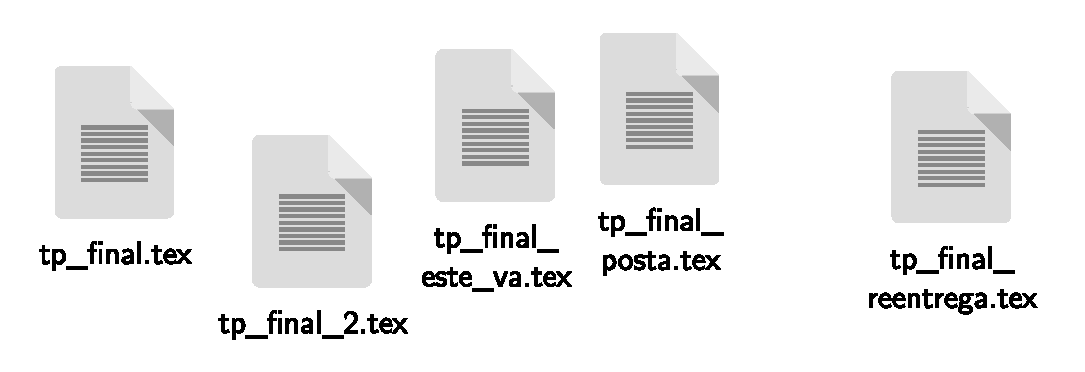
\includegraphics[height=1.5in]{images/caos.pdf}
        \end{center}
    \end{figure}

    \pause
    \begin{figure}[ht]
        \begin{center}
            
\includegraphics[height=1.5in]{images/horror.png}
        \end{center}
    \end{figure}
\end{frame}
\begin{frame}{Motivación 2/2}

    \begin{block}{Trabajando en grupo}
        \begin{itemize}
            \item Enviar cambios por mail, o
            \pause
            \item Enviar archivos por Discord, o
            \pause
            \item Sincronizar cambios por Google Docs.
        \end{itemize}
    \end{block}

    \pause
    \begin{figure}[h]
        \begin{center}
            
\includegraphics[height=1.5in]{images/horror.png}
        \end{center}
    \end{figure}

\end{frame}

\begin{frame}{¿Qué es un Sistema de Control de Versiones?}

	\begin{block}{}
 \begin{enumerate}
     \item Programas que permiten \textbf{manejar los cambios} en el código fuente de un proyecto a lo largo del tiempo.
     \item Llevan un \textbf{seguimiento} de las modificaciones que hacemos, y en caso de que nos equivoquemos, es posible volver atrás y comparar el código actual con versiones anteriores para ayudar a arreglar el error.
     \item Permiten que distintas personas modifiquen el código a la vez y \textbf{compartan los cambios}.
 \end{enumerate}

	\end{block}

 %   \pause
 %    \begin{resumen}{Es decir, permiten...}
 %        \begin{itemize}
 %            \item Arreglar \textit{accidentes} y volver a versiones anteriores del código.
 %            \item Compartir código con otras personas.
 %        \end{itemize}
	% \end{resumen}

\end{frame}

\begin{frame}{¿Qué es Git? 1/2}

	\begin{block}{}
 \begin{itemize}
     	\item Sistema de Control de Versiones \textbf{distribuido y de código abierto}.
  
        \item Con énfasis en la \textbf{performance} (para manejar proyectos muy grandes), \textbf{seguridad} y \textbf{flexibilidad}.
        
        \item Amplio conjunto de comandos que permiten realizar operaciones de alto y bajo nivel.

        \item Mantiene una copia local completa del proyecto.
 \end{itemize}

	\end{block}

    \begin{figure}[ht]
        \begin{center}
            
\includegraphics[height=1.5in]{images/logo-git.pdf}
        \end{center}
    \end{figure}
\end{frame}

\begin{frame}{¿Qué es Git? 2/2}
    \begin{center}
        \begin{block}{GIT - the stupid content tracker}

            "git" can mean anything, depending on your mood.
            
             - \textbf{random three-letter combination that is pronounceable}, and not actually used by any common UNIX command.  The fact that it is a mispronunciation of "get" may or may not be relevant.\newline
             - \textbf{stupid}. contemptible and despicable. simple. Take your pick from the dictionary of slang.\newline
             - \textbf{"global information tracker"}: you're in a good mood, and it actually works for you. Angels sing, and a light suddenly fills the room. \newline
             - \textbf{"goddamn idiotic truckload of sh*t"}: when it breaks
        \end{block}
    \end{center}
    \pause
    \textit{ - Mensaje del commit de Linus Torvalds agregando el README al repositorio Git de Git (uf)}
    
\end{frame}

% revisar 
% se podría intercalar el status en todos los pasos
% \begin{frame}[t]{¿Cómo funciona Git?}
%     \begin{center}
%         \begin{block}{Sistema de \textit{Snapshots}}
%         \begin{enumerate}
%             \item Piensa a los datos como una serie de 'fotos' del sistema de archivos.
%             \item Con cada commit, o cada vez que guardas el estado del repo, saca una 'foto' del mismo y guarda una referencia a esa foto.
%             \item Si los archivos no cambian, no saca ninguna foto, solo mira la última.
            
%         \end{enumerate}

%         \end{block}

%         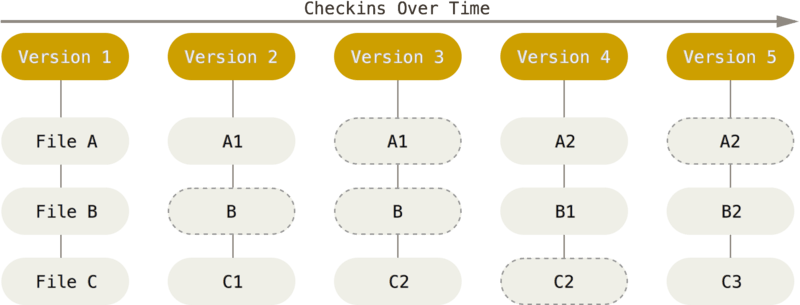
\includegraphics[width=4in]{images/snapshots.png}
%     \end{center}
    
%\end{frame}




\begin{frame}[t]{Creando un repositorio vacío}
    \begin{comando}
        git init
    \end{comando}

    \pause
    \begin{block}{}
        Crea un repositorio local vacío. Un lienzo en blanco, por así decirlo.
        \begin{enumerate}
            \item Nos paramos en el directorio que queremos convertir en un repositorio.
            \item Ejecutamos \texttt{git init}.
        \end{enumerate}
        Esto crea un subdirectorio \textit{.git} que tiene todos los archivos necesarios de Git.
    \end{block}
    \pause
    \begin{ejercicio}{Ejercicio}
        En el escritorio, creen una carpeta nueva con el nombre de su repositorio. Dentro de ella, ejecuten \texttt{git init}.
    \end{ejercicio}
\end{frame}
\begin{frame}[fragile, t]{¿Está preparado, confirmado o ninguna de las dos?}
    \begin{comando}
        git status
    \end{comando}
        \begin{block}{Output de ejemplo}
            \begin{center}
            \texttt{nothing to commit (create/copy files and use "git add" to track)}
            \end{center}
        \end{block}
    \pause
    \begin{ejercicio}{Ejercicio}
        Crear un nuevo archivo en nuestro repositorio y ejecutar \textit{git status} y vean como cambia el mensaje.
    \end{ejercicio}

\end{frame}

\begin{frame}[fragile, t]{¿Está preparado, confirmado o ninguna de las dos?}
    \begin{comando}
        git status
    \end{comando}
    \begin{block}{Output de ejemplo}
            \begin{center}
            \texttt{Untracked files:
  (use "git add <file>..." to include in what will be committed) \\archivo}
            \end{center}
        \end{block}
\begin{ejercicio}{Ejercicio}
    Ejecuten el comando que les sugiere \textit{git} para incluír el archivo. Hagan \textit{git status}.
\end{ejercicio}
\end{frame}

\begin{frame}[fragile, t]{¿Está preparado, confirmado o ninguna de las dos?}
    \begin{comando}
        git status
    \end{comando}
    \begin{block}{Output de ejemplo}
            \begin{center}
            \texttt{Changes to be committed:
  (use "git rm --cached <file>..." to unstage)
        \\new file:  archivo}
            \end{center}
        \end{block}
   \begin{block}{}
       Con esto vemos que \textit{git} ahora conoce al nuevo archivo, y lo va a tener en cuenta cuando hagamos un \textit{commit} proximamente.
   \end{block}     
\end{frame}

\begin{frame}{Estados de un archivo}

    \begin{block}{Los cuatro estados de los archivos}
            \begin{enumerate}
    \item Untracked = Sin seguimiento
    \item Unmodified = Sin modificar
    \item Modified = Modificado
    \item Staged, to be commited = Confirmado
    \end{enumerate}
    \end{block}
    \begin{center}
        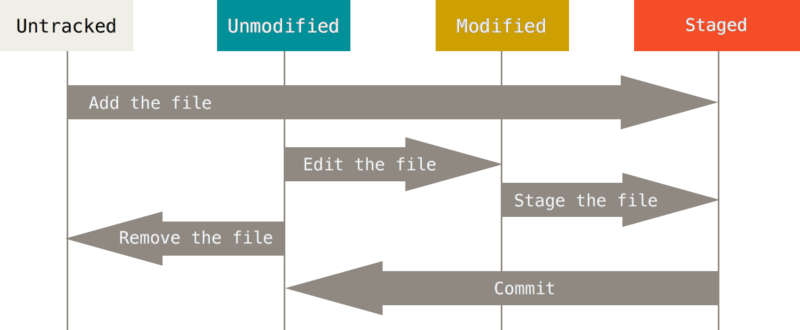
\includegraphics[width=4in]{images/lifecycle.png}
    \end{center}    
\end{frame}

\begin{frame}[t]{Confirmando cambios}
    \begin{comando}
        git commit
    \end{comando}

    \pause
    \begin{block}{}
        Una vez que tenemos ciertos cambios marcados con \textit{add}, podemos confirmarlos
        ejecutando \texttt{git commit -m "mensaje"}.

        \vspace{0.5em}

        Donde \texttt{[mensaje]} es una breve descripción de los cambios que acabamos de confirmar.
    \end{block}

    \pause
    \vspace{1em}
    \pause
    \begin{ejercicio}{Ejercicio}
        Hagan el \textit{commit} que venían preparando y elijan un mensaje. Luego hagan \textit{git status}.
    \end{ejercicio}
\end{frame}



\begin{frame}[fragile]{Configuraciones iniciales}

    \begin{block}{Tu identidad}
        Es importante establecer nuestro \textbf{nombre y email} en nuestro repositorio, ya que estos van a ir asociados con los cambios que hagamos:

        \vspace{0.5em}

        \texttt{git config --global user.name "Guybrush Threepwood"}

        \texttt{git config --global user.email guybrush@example.com}


    También se puede omitir el flag \texttt{--global} para que las credenciales apliquen solo al repositorio en el que estamos trabajando.
        \end{block}
\end{frame}

\begin{frame}{Historial}
 \begin{comando}
     git log
 \end{comando}
 \pause
 \begin{block}{}
     Este comando nos sirve para ver el historial de cambios, o commits. Además nos dice quién hizo cada cosa, cuando, y su correo electrónico.
     
 \end{block}
    \begin{ejercicio}{Ejercicio}
        Fíjense quien es el autor de sus cambios anteriores...
        
        Después, hagan algún otro \texttt{commit} y miren que pasa.
    \end{ejercicio}
\end{frame}

\begin{frame}[t]{¡No seas vago con los mensajes!}

    \begin{figure}[ht]
        \begin{center}
            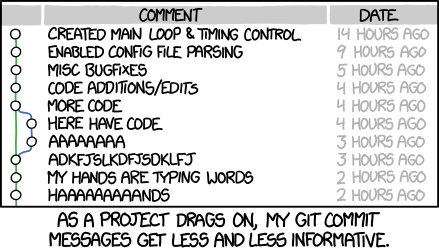
\includegraphics[height=2in]{images/xkcd-git-commit.png}
        \end{center}
        \caption{Fuente: \url{https://xkcd.com/1296/}}
    \end{figure}

\end{frame}
